%!TEX root = ../report.tex
\section{Results}
We have implemented the methods as described in the Implementation section.
Our project is not quite done, but the first results are visible in figure~\ref{fig:res}.

\begin{figure}[!th]
\hrule
\begin{center}
\vspace*{2ex}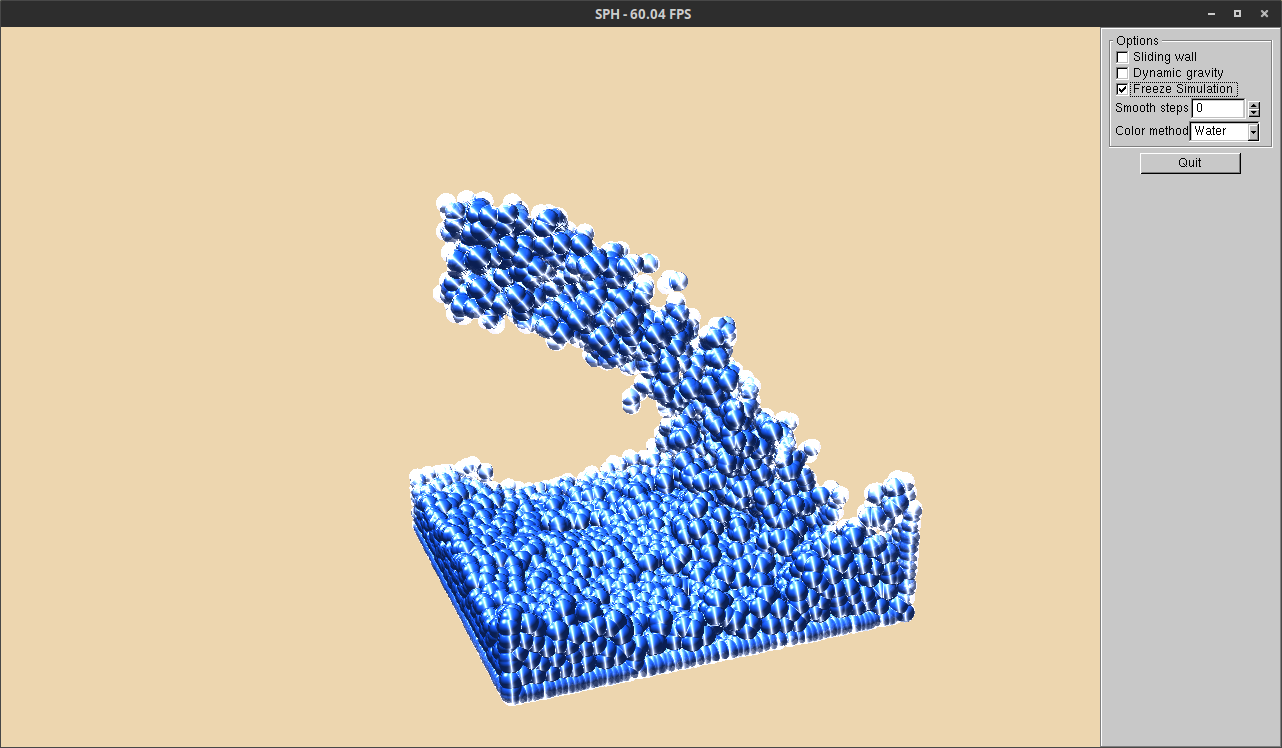
\includegraphics[width=0.48\textwidth,clip=true,trim=10cm 1cm 10cm 5cm]{pictures/colors_unsmoothed.png}
\end{center}
\caption{The SPH simulation with splatted point and Phong and Fresnel rendering without surface smoothing}
\label{fig:res} 
\vspace*{2ex}
\hrule
\end{figure}

\begin{figure}[!th]
\hrule
\begin{center}
\vspace*{2ex}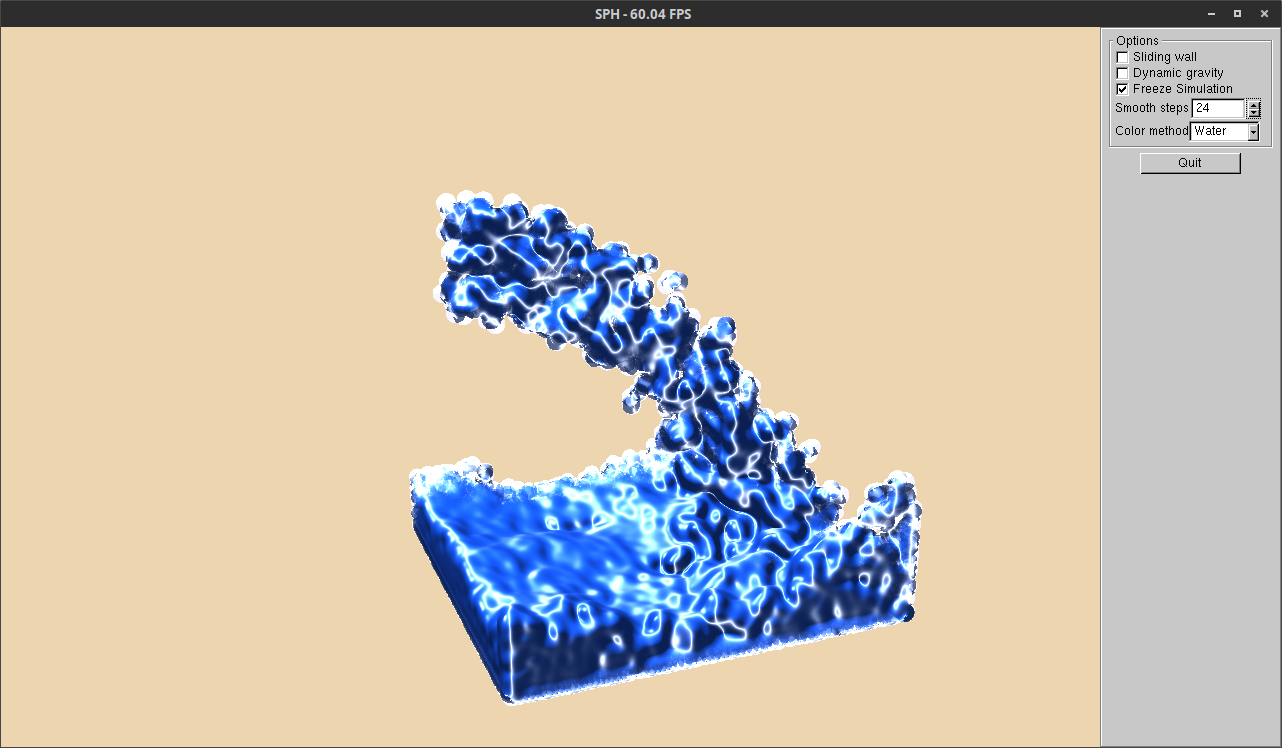
\includegraphics[width=0.48\textwidth,clip=true,trim=10cm 1cm 10cm 5cm]{pictures/colors_smoothed.png}
\end{center}
\caption{The same simulation visualized with 24 smooth steps}
\label{fig:res} 
\vspace*{2ex}
\hrule
\end{figure}


Currently, splatting the points and determining the normals per fragment works. Also parts of the rendering implementation are complete, but refraction of the water is lacking.
Moreover, thickness is currently not implemented, as well as noise and foam.
Most notably lacking is the smoothing pass. 

\section{Conclusion}
When the initial requirements for the realistic water rendering are considered it seems that the curvature flow way is a good fit.
\begin{itemize}
\item Given enough iterations of the fluid surface, a surface will become smooth and will have no sharp discontinuities between particles.
\item It is possible to generate an imperfect surface by adding a noise texture to the surface and attaching it to particles. This will distort the surface a little bit and will create an imperfect, and more natural surface
\item It takes into account attenuation of colors based on the depth of the fluids and submerged objects. Moreover, foam can be added for an added realistic effect.
\end{itemize}
Besides that it can produce a natural rendering of a fluid surface, it is also fast. 
It can render a smooth surface from thousands of particles and still have an acceptable framerate. 

Even so, there is still room for improvement with this method. There are possibilities to exploit parallelism in the form of GPGPU processing in order to improve performance.
Moreover, this paper is currently several years old and large advancements have been made in the capabilities of graphics frameworks as OpenGL and DirectX.
These new features could be exploited for a higher performance and better visualization.

Also, our current implementation is not perfect. Several features as described in the paper are missing, thus reducing the realism and immersion. Improvements can be made by implementing features as thickness, noise and foam.